\section{Introduction}

\subsection{Numerical Methods compared to Symbolic Methods}

Engineering design for given specifications  often requires the solution of nonlinear systems of equations after defining component element parameters.
%functional specification component parameters. 
Usually for the determination of the wanted variables numeric optimizing procedures are used, which do not function reliably however already for small design problems with a comparatively small number of unknowns. 
Above all, the complexity order of many usual optimizing algorithms is exponentially dependent on the number of variables, which  cause problems  (a problem, known as the {\em curse of dimensionality} \cite{Michalewicz} is), then the selection of suitable initial values, the unwanted finding of locally instead of global optima and the principle-conditioned behavior during the solution of systems of equations with degrees of freedom, with which a uniqueness of the solution vector is not realizable. 

The best procedure for the accomplishment of a design task would basically be a complete analytic solution of the corresponding system of equations. Analytic functions, which describe explicitly the wanted values as functions of the specification parameters, would have to be determined only once and would be available afterwards to the arbitrarily frequent evaluation with modified parameters, e.g. within design data bases of CAD systems. Besides analytic dimensioning formulas clarify qualitatively functional connections between the element values and the specifications and reveal in the relevant cases  the existence of degrees of freedom. 
Since there exists however no generally accepted procedures for the solution of nonlinear systems of equations and in those special cases, in which symbolic solutions can be calculated, the complexity of the results far exceeds by hand calculation to mastering frameworks, the analytic handling of very low dimensioning problems plays so far a subordinated role. 

With the help of modern, efficient computer algebra systems, which are able to manipulate   systems of symbolic equations algebraically, and solve using arbitrary variables, become some of these problem categories nevertheless accessible for an analytic handling. In particular such problems, specified above, which require the solution of linear or multivariate polynomial systems.
Examples of such applications are within many fields of engineering sciences, such as the design of analog electronic circuits, regulation-technical problems, engineering mechanics and robotics \cite{Pfalzgraf}.



\subsection[Examples of Areas of Application of Symbolic Design Methods]{Examples of Areas of Application of Symbolic Design Methods}

On the basis of the following two examples we demonstrate some areas of application of symbolic methods. At the same time, the concrete requirements should be worked out at them, which must be considered with respect to the development of  a universal solution algorithm for symbolic systems of equations .


\begin{example}{TM}

The first example concerns  a simple task  of engineering mechanics. Given is the two rod truss represented in figure \ref{Stabzweischlag}, \cite[S.~112]{Brommundt}, at which under the angle $\gamma$ opposite the horizontals the force $F$ attacks in the point $C$. The rods form the angles $\alpha$ and $\beta$ with the horizontals, the height of the triangle stretched by the rods are denoted with $c$. The  Cross sections  $A_1$ und $A_2$  of the two rods are squares with the side lengths $h_1$ und $h_2$. The modulus of elasticity of the used material be $E$. 

\begin {figure} [htbp]
\begin {center}
\centerline{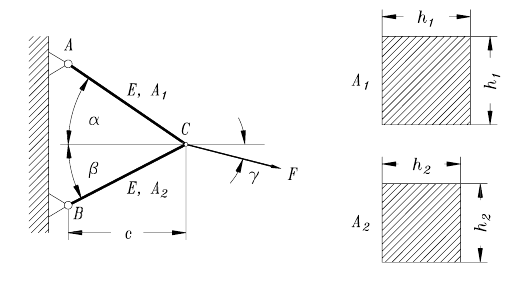
\includegraphics[height=4cm]{zweischl.png}}
\caption {\begin {minipage} [h] {10cm}% --- TABLE
 loaded two rod truss (in German: 'Stabzweischlag')
\label{Stabzweischlag}
\end {minipage}
}%small
\end {center}
\end {figure}
%\inbildpsf{Loaded double bar impact}{zweischl.png}{86mm}{Double bar impact}
Due to the load by the strength $F$  the truss deforms in such a way, that the point of the triangle in relation to the unloaded status around the vector $(u,w)^T$ shifts, see figure  \ref{Belastung}. On the assumption that the rod lengths variations are small due to the load in relation to the original lengths, now  the cross section dimensions $h_1$ and $h_2$ of the rods are to be determined  in such a way, that for given $F$, $\alpha$, $\beta$, $\gamma$, $c$ and $E$ there results exactly one prescribed shift $(u,w)^T$, i.e. we look for

\begin{equation}
\cvec{a_1\\a_2} = \f( F, \alpha, \beta, \gamma, c, E, u, w).
\end{equation} 

\newpage
\begin {figure} [htbp]
\begin {center}
\centerline{\includegraphics[height=4.4cm]{belastg.png}}
\caption {\begin {minipage} [h] {10cm}% --- TABLE
elastically deformed two rod hit
\label{Belastung}
\end {minipage}
}%small
\end {center}
\end {figure}
%\inbildpsf{Elastisch verformter Stabzweischlag}{belastg.eps}{105mm}{Belastung}

\noindent {\bf Solution:}  From the static balance conditions at the point $C$ it follows after figure \ref{Freischnitt}
\begin{eqnarray}
\sum F_{xi} = 0 & \Longrightarrow & 
  F \cos \gamma - S_1 \cos \alpha - S_2 \cos \beta = 0, \label{TMGS1}\\
\sum F_{zi} = 0 & \Longrightarrow & 
  F \sin \gamma - S_1 \sin \alpha + S_2 \sin \beta = 0.
\end{eqnarray}

\begin {figure} [htbp]
\begin {center}
\centerline{\includegraphics[height=4.4cm]{kraefte.png}}
\caption {\begin {minipage} [h] {10cm}% --- TABLE
balance of forces at point $C$
\label{Freischnitt}
\end {minipage}
}%small
\end {center}
\end {figure}

%\inbildpsf{Kr"aftegleichgewicht am Punkt $C$}{kraefte.eps}{44mm}{Freischnitt}

\noindent 
The material equations for the variations of the rod lengths are
\begin{eqnarray}
\Delta l_1 &=& \frac{S_1 l_1}{E A_1}, \\
\Delta l_2 &=& \frac{S_2 l_2}{E A_2},
\end{eqnarray}
whereby for the rod lengths $l_1$ und $l_2$ and for the cross-section areas $A_1$ und $A_2$ we have
\begin{eqnarray}
l_1 &=& \frac{c}{\cos \alpha} \label{l1} \\
l_2 &=& \frac{c}{\cos \beta}  \label{l2} \\
A_1 &=& h_1^2, \\
A_2 &=& h_2^2.
\end{eqnarray}


\begin {figure} [htbp]
\begin {center}
\centerline{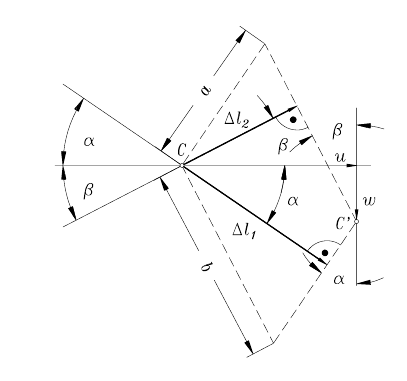
\includegraphics[height=6.4cm]{vschplan.png}}
\caption {\begin {minipage} [h] {10cm}% --- TABLE
displacement plan
\label{Verschiebungsplan}
\end {minipage}
}%small
\end {center}
\end {figure}
%\inbildpsf{Verschiebungsplan}{vschplan .eps}{60mm}{Verschiebungsplan}

In the shift plan, drawn in figure \ref{Verschiebungsplan}, we replaced the circular arcs, on which the rod ends can move,  by the  tangents perpendicular to the  original rod directions. This is possible, because of the small geometry variations. For the side lengths of the dashed parallelogram we have 

\begin{eqnarray}
a &=& \frac{\Delta l_2}{\cos(90^\circ - \alpha - \beta)}
  = \frac{\Delta l_2}{\sin(\alpha + \beta)}, \\
b &=& \frac{\Delta l_1}{\cos(90^\circ - \alpha - \beta)}
  = \frac{\Delta l_1}{\sin(\alpha + \beta)}.
\end{eqnarray}
Therefore we have for the shifts $u$ und $v$ 
\begin{eqnarray}
u &=& a \sin \alpha + b \sin \beta, \\
v &=& -a \cos \alpha + b \cos \beta. \label{TMGS12}
\end{eqnarray}

The task is now, to solve the symbolic set of equations from the equations  (\ref{TMGS1}) bis (\ref{TMGS12}) for the unknowns $h_1$ and $h_2$ explicitly, whereby all unnecessary variables, i.e. $S_1$, $S_2$, $A_1$, $A_2$, $\Delta l_1$, $\Delta l_2$, $a$ und $b$, are to be eliminated.
\end{example}



\begin{example}{ET}

The second example originates from electro-technology and concerns the dimensioning of analog electronic circuits. For the two-stage transistor amplifier drawn in figure \ref{BJTAmp} \cite{Nuehrmann}, there are  symbolic dimensioning formulas  to be determined, which describe the values of the seven resistances 
$R_1 \, \ldots \, R_7$ as function of the operating voltage $V_{CC}$, of the small signal reinforcement $A$, of the input resistance $Z_i$ and the output resistance $Z_o$  of the circuit for numerically determined work points of the transistors:
\begin{equation} \label{Rdim}
\cvec{R_1\\\vdots\\R_7} = \f( V_{CC}, A, Z_i, Z_o ).
\end{equation}


\begin {figure} [htbp]
\begin {center}
\centerline{\includegraphics[height=6.4cm]{bjtamp.png}}
\caption {\begin {minipage} [h] {10cm}% --- TABLE
Two-stage transistor amplifier
\label{BJTAmp}
\end {minipage}
}%small
\end {center}
\end {figure}
%\inbildpsf{Zweistufiger Transistorverst"arker}{bjtamp.eps}{103mm}{BJTAmp}


\begin {figure} [htbp]
\begin {center}
\centerline{\includegraphics[height=6.4cm]{bjtampop.png}}
\caption {\begin {minipage} [h] {10cm}% --- TABLE
Working point equivalent circuit diagram of the amplifier with specified
transistor operating points
\label{BJTAmpOP}
\end {minipage}
}%small
\end {center}
\end {figure}
%\inbildpsf{Arbeitspunktersatzschaltbild des Verst"arkers mit festgelegten 
%Tran\-si\-stor-Ar\-beits\-punk\-ten}{bjtampop.eps}{96mm}{BJTAmpOP}
For this purpose, with the help of symbolic network analysis procedures \cite{RalfsDiss}  as well as symbolic approximation methods \cite{DA}, 
at first the (highly simplified)  transfer functions $A$, $Z_i$
and $Z_o$ in the pass band of the amplifier are calculated as functions of the elements parameters and the work point values.
\begin{eqnarray}
A   &=& \frac{145303681853 R_2}{145309663773 R_1}\label{BJTAmpA} \\
Z_i &=& R_7\\
Z_o &=& \frac{1675719398828125 \: R_2 \: R_7 
+ 394048139880824192 \: R_1 \: R_2}{136552890630303121408 \: R_1}
\label{BJTAmpZo}
\end{eqnarray}
The values of the resistances $R_1\, \ldots \, R_7$ do not only determine the small signal characteristics, but influence besides the work point adjustment of the circuit. Therefore the resistances
are to be dimensioned in such a way, that the small signal and the work point specifications are fulfilled  {\em at the same time}. For this reason, an  extensive sparse tablet set of equations  (\ref{BJTAmpSTA1}) -- (\ref{BJTAmpSTAn}) is added to the equations (\ref{BJTAmpA}) -- (\ref{BJTAmpZo}), which comes out from the work point alternate circuit diagram of the amplifier represented in figure \ref{BJTAmpOP}.
\begin{eqnarray}
I_{\rm VIN}+I_{\rm C1} & = & 0 \label{BJTAmpSTA1}\\
I_{\rm R7}+I_{\rm FIX2,Q1}-I_{\rm C1} & = & 0 \\
I_{\rm R2}+I_{\m R1}-I_{\rm FIX2,Q1}-I_{\rm FIX1,Q1} & = & 0 \\
I_{\rm R6}+I_{\rm FIX2,Q2}+I_{\rm FIX1,Q1} & = & 0 \\
-I_{\rm R7}+I_{\rm R5}+I_{\rm R4} & = & 0 \\
-I_{\rm R4}-I_{\rm FIX2,Q2}-I_{\rm FIX1,Q2}+I_{\rm C2} & = & 0 \\
I_{\rm R3}-I_{\rm R2}+I_{\rm FIX1,Q2} & = & 0 \\
I_{\rm VCC}-I_{\rm R6}-I_{\rm R3} & = & 0 \\
  \medskip
-V_{\rm VIN}+V_{\rm R1}+V_{\rm FIX2,Q1}+V_{\rm C1} & = & 0 \\
-V_{\rm R2}+V_{\rm FIX2,Q2}-V_{\rm FIX1,Q2}-V_{\rm FIX1,Q1} & = & 0 \\
-V_{\rm R6}+V_{\rm R3}+V_{\rm R2}+V_{\rm FIX1,Q1} & = & 0 \\
V_{\rm R7}+V_{\rm R4}-V_{\rm R2}-V_{\rm FIX2,Q1}-V_{\rm FIX1,Q2} & = & 0 \\
-V_{\rm VIN}+V_{\rm R7}+V_{\rm R5}+V_{\rm C1} & = & 0 \\
-V_{\rm VIN}+V_{\rm R2}+V_{\rm FIX2,Q1}+V_{\rm FIX1,Q2}+V_{\rm C2}
  +V_{\rm C1} & = & 0 \\
V_{\rm VCC}-V_{\rm VIN}+V_{\rm R6}+V_{\rm FIX2,Q1}-V_{\rm FIX1,Q1}
  +V_{\rm C1} & = & 0 \label{BJTAmpSTAlastlin} \\
  \medskip
R1 \cdot I_{\rm R1}-V_{\rm R1} & = & 0 \\
R2 \cdot I_{\rm R2}-V_{\rm R2} & = & 0 \\
R3 \cdot I_{\rm R3}-V_{\rm R3} & = & 0 \\
R4 \cdot I_{\rm R4}-V_{\rm R4} & = & 0 \\
R5 \cdot I_{\rm R5}-V_{\rm R5} & = & 0 \\
R6 \cdot I_{\rm R6}-V_{\rm R6} & = & 0 \\
R7 \cdot I_{\rm R7}-V_{\rm R7} & = & 0 \\
-I_{\rm C1} & = & 0 \\
-I_{\rm C2} & = & 0 \\
V_{\rm VIN} & = & 0 \label{BJTAmpSTAvin} \\
V_{\rm VCC} & = & VCC \\
V_{\rm FIX1,Q1} & = & 2.72 \\
V_{\rm FIX2,Q1} & = & 0.607 \\
V_{\rm FIX1,Q2} & = & 6.42 \\
V_{\rm FIX2,Q2} & = & 0.698 \\
I_{\rm FIX2,Q2} & = & 1.26 \cdot 10^{-5} \\
I_{\rm FIX1,Q2} & = & 0.00401 \\
I_{\rm FIX2,Q1} & = & 5.75 \cdot 10^{-7} \\
I_{\rm FIX1,Q1} & = & 1.11 \cdot 10^{-4} \label{BJTAmpSTAn}
\end{eqnarray}
For the determination of the wanted dimensioning regulations in the form (\ref{Rdim}) from the set of equations (\ref{BJTAmpA}) -- (\ref{BJTAmpSTAn})  all branch voltages and flows $V_{??}$ and $I_{??}$ are to be eliminated
 and the remaining equations solved for the resistances $R_1 \, \ldots \, R_7$.
\end{example}

\section[ Conventional Equation Solver]{Limits of the Application of Conventional Equation Solvers}

If an attempt is undertaken to use the standard routines of well-known commercial computer algebra systems like Macsyma \cite{Macsyma}  or Mathematica \cite{Wolfram} for the solution of the systems of equations from the two examples from above, then in the case of use of  Maxima/Macsyma in the example  \ref{TM} we get usually the following typeof  result, like here:

\begin{literatim}{|}
(COM1) Solve(
  [
    F*cos(gamma) - S1*cos(alpha) - S2*cos(beta) = 0,
    F*sin(gamma) - S1*sin(alpha) + S2*sin(beta) = 0,
    Delta_l1 = l1*S1/(E*A1),
    Delta_l2 = l2*S2/(E*A2),
    l1 = c/cos(alpha),
    l2 = c/cos(beta),
    a = Delta_l2/sin(alpha+beta),
    b = Delta_l1/sin(alpha+beta),
    u = a*sin(alpha) + b*sin(beta),
    w = -a*cos(alpha) + b*cos(beta),
    A1 = h1^2,
    A2 = h2^2
  ],
  [h1, h2]
);
(D1) []
\end{literatim}

This behavior of the computer algebra systems is explained with the fact, that the systems of equations to be solved for the interesting variables $h_1$ and $h_2$ are regarded as over-determined, because the equation solvers cannot be given additional information about (after possibility) the {\em to be eliminated} variables ($S_1$, $S_2$, $A_1$, $A_2$, $\Delta l_1$,
$\Delta l_2$, $a$, $b$) resp.  the parameters of the system ($F$, $\alpha$, $\beta$, $\gamma$,
$c$, $E$, $u$, $w$), which should {\em not be eliminated under any circumstances}. 

A possible way out for the equation solvers consists in letting them determine also solutions for the not interesting variables. However, this is not always feasible and usually very inefficient, because in some cases much computing time is necessary for the calculation of variables, which have no impact on the looked for unknowns. Even at all, no solution is found, if there is no analytic solution for only one not interesting variable. The latter applies for example to the following system of equations, if only the solutions for $x$ and $y$ are looked for:

\begin{eqnarray}
x  + y      &=& 1  \label{lin1} \\
2x - y      &=& 5  \label{lin2} \\
yz + \sin z &=& 1. \label{nlin3}
\end{eqnarray}
From the two linear equations (\ref{lin1}) and (\ref{lin2}) the solutions  $x = 2$ and $y = -1$ are determined directly, not in the contradiction with the remaining nonlinear equation (\ref{nlin3}). Maxima does not detects this circumstance and gives back only error messages -- 
 in the first attempt ({\tt COM3}) due to  the apparent over-determinacy of the system, in the second attempt ({\tt
COM4}) due to the analytically not solvable third equation:
\begin{literatim}{|}
(COM2) Eq : [x + y = 1, 2*x - y = 5, y*z + sin(z) = 1]$
(COM3) Solve( Eq, [x, y] );
Inconsistent equations:  (3)
(COM4) Solve( Eq, [x, y, z] );
ALGSYS cannot solve - system too complicated.
\end{literatim}

\section[Requirements to an Symbolic Equation Solver]%
{\label{SolverAnforderungen}Requirements to an Universal Symbolic Equation Solver}

For the symbolic solution of the system of  equations, it is necessary that the  \verb+Solve+ function in none of the two above cases aborts prematurely. In the first case, after a consistency check with equation (\ref{nlin3}), the solutions $x$ and $y$ should be returned. 
In the latter case it is to be desired, that beside the analytically calculated solutions, the remaining equations, for which no such solutions could be found, should be  returned additionally in implicit form -- so that these could be solved with numerical methods. An adequate response to the command \verb+COM4+ would then be e.g.\ an output of the form
\begin{displaymath}
\left[ x = 2, \,\, y = -1, \,\, -z + \sin z = 1 \right].
\end{displaymath}  

The functions for the solution of sets of equations, provided by Maxima, are not modifiable without access to the system core in the way that they show the required behavior. The aim of this report is therefore a conceptualization and implementation of a universal symbolic equation solver, which is based on  Maxima standard routines, which is able to solve sets of equations of the type stated in the examples after any subset of all variables. Or at least by elimination of not necessary variables as much as possible  to do a large symbolic preprocessing of the equations, so that numeric optimizing procedures do have  only be applied to a small, analytically not solvable nonlinear core of the system. 

Apart from this general objective, detailed requirements can be derived for the developed program  from some well-known facts and a series of observations, which came from the examples \ref{TM} and \ref{ET}  as well as the system of equations (\ref{lin1}) -- (\ref{nlin3}):

\begin{enumerate}
\item Usually only the solution for some few variables is asked for, all other unknowns  are to be eliminated.

\item 
The sets of equations which are to be solved can be one times or more times parameterized.

\item 
It is not  guaranteed by any means, that the parameters are  independent from each other, i.e. it is possible that a system of equations has only a solution, if certain arithmetic forced conditions between some parameters are kept.

\item The systems of equations contain often simple, direct assignments of the form  $x_i = \const$, see equations (\ref{l1}) and 
(\ref{l2}) or (\ref{BJTAmpSTAvin}) -- (\ref{BJTAmpSTAn}).

\item A substantial proportion of the equations to be solved, is linear with respect to a not directly evident subset of all variables, see equations  (\ref{BJTAmpSTA1}) -- (\ref{BJTAmpSTAlastlin})which are linear with respect to all $V_{??}$ und $I_{??}$.

\item  The systems can contain degrees of freedom.

\item 
There exists no generally valid solution procedures for nonlinear equations and systems of equations.

\item 
Nonlinear equations can be unsolvable (contradictory), or have unique  or multiple solutions with finite or infinite solution varieties.

\item Not always, all members of the multiple solution set are consistent with the remaining equations.

\item  For many nonlinear equations there exists no analytic solutions, see equation (\ref{nlin3}).
\end{enumerate}


From these statements the following requirements results corresponding to the points  above::


\begin{enumerate}
\item The program should solve systems of equations only so far, as it is absolutely necessary for the determination of the individual variables. Calculated solutions are to be checked for possible contradictions with respect to the remaining equations.

\item 
Looked for variables and parameters must to be processed separately from each other.  Under any circumstances, parameters may not be  eliminated -- in contrast to not interesting variables.

\item If dependencies between parameters are detected, then the program run must continued under consideration and storage of the appropriate force conditions, if  desired by the user.

\item \label{AnfImmed}
Direct assignments should be looked for  and executed directly at the beginning of the program run, in order to reduce the scope of the remaining system of equations as far as possible and with little effort.

\item \label{AnfLinear}
Because there exists  efficient, closed solution procedures for linear equations, it is advisable to search the system of equations repeatedly for linear blocks, to solve these and put the results into the remaining  equations, until no more linear parts of equations are present.

\item 
Degrees of freedom are to be expressed automatically in variables selected by the program.

\item \label{AnfNonlinear}
The solution of nonlinear equations must be controlled with the help of heuristic evaluation strategies.

\item 
In case of multiple solutions with finite varieties, each individual solution path is separately recursively to be pursued.

\item 
Multiple solutions, which are inconsistent with the remaining equations, must be detected and the corresponding solution path rejected.

\item 
As was already required at the beginning of the section,  equations not analytically solvable should not lead to the abort of the program. Instead the system of equations should be brought  on triangle form is as far as possible  and the  remaining, not solvable equations returned along with the partial solutions determined up to then.

\end{enumerate}


% ================================================================= TO DO :

\section{== STOP/TO DO== Extraktion und L"osung linearer Gleichungen}

Zwar sind bei technischen Aufgabenstellungen die zu l"osenden Gleichungen
zumeist nichtlinear, doch enthalten die betreffenden Systeme h"aufig gro"se
lineare Teilbl"ocke. Da lineare Gleichungssysteme sehr effizient mit Hilfe
der Gau"s-Elimination simultan gel"ost werden k"onnen, empfiehlt es sich, vor
der L"osung der nichtlinearen Gleichungen zun"achst den linearen Anteil des
Systems separat zu verarbeiten. Selbst wenn eine vollst"andige analytische
Aufl"osung des gesamten nichtlinearen Systems nach allen gesuchten Variablen
nicht  erreicht werden kann, ist es dennoch sinnvoll, durch Elimination der
linearen Variablen und Gleichungen das System auf einen nur noch kleinen,
nicht mehr analytisch l"osbaren Kern zu reduzieren, dessen numerische L"osung
wesentlich weniger aufwendig ist, als eine auf dem vollst"andigen System
durchgef"uhrte Optimierung.

Die unter Punkt \ref{AnfLinear} geforderte iterative L"osung linearer 
Teilsysteme des gesamten Gleichungssystems ist insofern keine triviale
Aufgabe, als da"s weder die betreffenden Gleichungen noch die Teilmenge
der Variablen, bez"uglich der diese Gleichungen linear sind, von
vornherein bekannt sind. Deshalb mu"s eine Suchstrategie gefunden 
werden, die (aus Effizienzgr"unden m"oglichst gro"se) lineare
Gleichungs- und Variablenbl"ocke aus einem beliebigen nichtlinearen
Gleichungssystem extrahiert.

\subsection{\label{intuitive}Intuitive Vorgehensweisen zur Suche
linearer Gleichungen}

Zur Verdeutlichung der Aufgabenstellung wird das folgende nichtlineare
Gleichungssystem herangezogen, das nach den Variablen $x$, $y$ und $z$ 
zu l"osen sei.
\begin{eqnarray}
 x + 2y -    z &=&  6 \label{linearxyz} \\
2x + yz -  z^2 &=& -1 \label{linearx}   \\
3x -  y + 2z^2 &=&  3 \label{linearxy}
\end{eqnarray}
Auf den ersten Blick ist nur die Gleichung (\ref{linearxyz}) linear, und
zwar in bezug auf alle drei Variablen. Bei Verwendung eines einfachen 
Suchalgorithmus, der ausschlie"slich solche vollst"andig linearen
Gleichungen findet, kann in diesem Fall maximal eine Variable nach
entsprechender Aufl"osung von (\ref{linearxyz}), z.B. nach $x$, aus den
beiden restlichen Gleichungen eliminiert werden.

Eine genauere Betrachtung der Gleichungen offenbart aber eine bessere 
Alternative. Nach der Entfernung von Gleichung (\ref{linearx}) und dem
Verschieben der von $z$ abh"angigen Terme auf die rechten Seiten der
Gleichungen (\ref{linearxyz}) und (\ref{linearxy}) entstehen {\em zwei}
in den Variablen $x$ und $y$ lineare Gleichungen:
\begin{eqnarray}
 x + 2y &=& 6 + z,    \label{linsub1} \\
3x -  y &=& 3 - 2z^2. \label{linsub2}
\end{eqnarray}
Deren simultane Inversion f"uhrt zu den in $z$ parametrisierten 
L"osungen
\begin{eqnarray}
x &=& -\frac{1}{7} \left( 4z^2 -  z - 12  \right), \\
y &=&  \frac{1}{7} \left( 2z^2 + 3z + 15  \right),
\end{eqnarray}
nach deren Einsetzen in (\ref{linearx}) nur noch {\em eine} zu 
l"osende nichtlineare Gleichung verbleibt:
\begin{equation}
2 z^3 - 12 z^2 + 17 z + 31 = 0.
\end{equation}
Angesichts der Tatsache, da"s bei der zweiten Variante in nur einer
Iteration zwei Unbekannte gleichzeitig bestimmt werden konnten, ist
letztere Vorgehensweise der zuerst angewendeten Suche nach vollst"andig 
linearen Gleichungen trotz des zus"atzlichen Umformungsaufwandes
vorzuziehen. Dies gilt insbesondere dann, wenn ein Gleichungssystem
"uberhaupt keine Gleichungen enth"alt, in denen alle beteiligten
Variablen in rein linearer Form auftreten. Das zur Extraktion linearer 
Teilsysteme verwendete Verfahren sollte daher beide demonstrierten
Operationen zur Beseitigung nichtlinearer Gleichungsanteile miteinander
verbinden:
\begin{enumerate}
\item Entfernung einzelner nichtlinearer Gleichungen
\item Verschieben von in nichtlinearen Termen auftretenden Variablen auf 
die rechten Seiten der Gleichungen 
\end{enumerate}
Durch eine ausgewogene Kombination der zwei Operationen kann erreicht
werden, da"s die resultierenden linearen Teilsysteme maximale Gr"o"se haben 
und --- oft zumindest ann"ahernd --- quadratisch sind.

\subsection{\label{HeurAlgoLin}Ein heuristischer Algorithmus zur Suche
linearer Gleichungen}

F"ur eine Rechnerimplementation mu"s eine solche vom Menschen intuitiv 
durchgef"uhrte Suche nach linearen Gleichungsbl"ocken systematisiert und
algorithmisch formuliert werden. Da der Begriff {\em lineares
Teilgleichungssystem}, wie anhand der unterschiedlichen 
L"osungsm"oglichkeiten ersichtlich ist, das gew"unschte Resultat nicht
in eindeutiger Weise definiert, wurde eine heuristische Strategie zur 
Nachahmung der intuitiven Vorgehensweise entwickelt. Diese Strategie
wird  zum Vergleich der Ergebnisse an dem schon betrachteten System
(\ref{linearxyz}) -- (\ref{linearxy}) demonstriert.

F"ur das Gleichungssystem wird zun"achst eine Tabelle aufgestellt, deren
Zeilen den Gleichungen und deren Spalten den Variablen zugeordnet sind.
Der Eintrag an der Position $(i,j)$ der Tabelle enth"alt f"ur die  
Gleichung $i$ den Koeffizienten

%\footnote{Macsyma stellt zur Bestimmung
%der Koeffizienten rationaler Ausdr"ucke den Befehl \verb+RATCOEFF+ zur
%Verf"ugung.} 

bez"uglich des linearen Gliedes, d.h. der ersten Potenz,
der Variablen $x_j$. Ist wie f"ur $z$ in Gleichung (\ref{linearxy})
kein Term in erster Potenz vorhanden oder tritt dieser als Argument
nicht polynomialer Funktionen auf (z.B. $\sin x$ oder $\sqrt x$), so
wird die zugeh"orige Position mit einem Kreuz ($\times$) markiert.
\begin{displaymath}
\begin{array}{l|rrr}
               & x &  y &  z \\
\hline
\mbox{Gl.~} 1) & 1 &  2 & -1 \\
\mbox{Gl.~} 2) & 2 &  z &  y \\
\mbox{Gl.~} 3) & 3 & -1 & \times 
\end{array}
\end{displaymath}
Dieser Tabelle wird eine zweite, gleich gro"se Bewertungsmatrix
zugeordnet, deren Eintr"age gleich Null sind, wenn der korrespondierende
Eintrag in der Koeffiziententabelle eine Konstante ist, und gleich Eins,
wenn der betreffende lineare Koeffizient gesuchte Variablen enth"alt oder nicht
existiert ($\times$). Au"serdem werden an den R"andern der Matrix die 
Zeilen- und Spaltensummen notiert, sowie unter den Summenzeichen rechts 
oben und links unten respektive die Zeilensumme der Spaltensummen ($\sum 
S$) und die Spaltensumme der Zeilensummen ($\sum Z$).
\begin{equation} \label{linbewmat}
\begin{array}{rr|rrr|c}
       &   & x & y & z & \sum S \\
       &   & 0 & 1 & 2 &      3 \\
\hline
  1)   & 0 & 0 & 0 & 0 &        \\
  2)   & 2 & 0 & 1 & 1 &        \\
  3)   & 1 & 0 & 0 & 1 &        \\
\hline
\sum Z & 3 &   &   &   &
\end{array}
\end{equation}
Offensichtlich entsprechen die Eins-Elemente in der Bewertungsmatrix 
genau den unerw"unschten nichtlinearen Anteilen im Gleichungssystem. 
Ein lineares Teilgleichungssystem und die zugeh"origen Variablen sind
dann gefunden, wenn mit einer Folge der am Ende von
Abschnitt~\ref{intuitive} aufgef"uhrten Operationen alle Einsen
beseitigt wurden. "Ubertragen auf Manipulationen der Bewertungsmatrix
entspricht dabei die 1.\ Operation dem Streichen der zu einer bestimmten
Gleichung geh"origen Zeile. Die 2.\ Operation ist "aquivalent zur
Entfernung der einer Variablen zugeordneten Spalte. Das lineare 
Teilsystem besteht anschlie"send aus denjenigen Gleichungen und 
Variablen, deren Zeilen und Spalten nicht aus der Matrix entfernt
wurden.

Die Reduktion der Bewertungsmatrix~(\ref{linbewmat}) zu einer Nullmatrix 
kann auf genau drei verschiedene Weisen erfolgen:
\begin{enumerate}
\item Streichen der Zeilen 2) und 3),
\item Streichen der Spalten $y$ und $z$,
\item Streichen der Zeile 2) und der Spalte $z$.
\end{enumerate}
Der Forderung nach maximaler Gr"o"se und m"oglichst quadratischer Form 
der linearen Gleichungsbl"ocke ist direkt auf die zu erzielenden
Eigenschaften der Nullmatrix "ubertragbar. In diesem Sinne ist die 
letztgenannte der drei Optionen optimal, denn sie liefert das schon im
vorigen Abschnitt als bestm"ogliche L"osung erkannte System 
(\ref{linsub1}) -- (\ref{linsub2}). Die beiden anderen M"oglichkeiten 
f"uhren dagegen zu der unterbestimmten Gleichung (\ref{linearxyz}) bzw.\
zu einem "uberbestimmten $3 \times 1$-System in $x$.

Die Suche nach einer optimalen Folge von Zeilen- und 
Spaltenstreichungen ist ein komplexes kombinatorisches Problem. Um den 
damit verbundenen Aufwand zu vermeiden, wird zur Bestimmung der im 
jeweiligen Schritt zu entfernenden Zeile oder Spalte ein heuristisches,
lokales Entscheidungskriterium, d.h. eine {\em Greedy}-Strategie 
\cite{Foulds}, verwendet: Es wird die Zeile oder Spalte gestrichen, die 
die meisten Einsen enth"alt, also diejenige mit der gr"o"sten Zeilen- 
bzw.\ Spaltensumme. Dieses Kriterium liefert jedoch noch keine 
eindeutige Aussage, wenn
\begin{itemize}
\item zwei oder mehr Zeilen die gleiche (gr"o"ste) Zeilensumme 
haben,
\item zwei oder mehr Spalten die gleiche (gr"o"ste) Spaltensumme 
haben,
\item oder wenn die Summen der h"ochstbewerteten Zeile und der
h"ochstbewerteten Spalte identisch sind.
\end{itemize}
In den ersten beiden F"allen kann aus den betreffenden Zeilen oder 
Spalten eine beliebige ausgew"ahlt werden, in der Regel ist
dies der Einfachheit halber die jeweils zuerst gefundene mit maximaler
Bewertung. 

Der dritte Fall tritt im vorliegenden Beispiel auf. In der 
Bewertungsmatrix (\ref{linbewmat}) besitzen sowohl die Zeile 3) als auch 
die Spalte $z$ die maximale Summe $2$. Zu Beginn werde aus beiden 
M"oglichkeiten willk"urlich die Streichung der Zeile ausgew"ahlt, so da"s 
sich im n"achsten Schritt folgende Bewertungsmatrix ergibt:
\begin{equation}
\begin{array}{rr|rrr|c}
       &   & x & y & z & \sum S\\
       &   & 0 & 0 & 1 &    1  \\
\hline
  1)   & 0 & 0 & 0 & 0 &       \\
  3)   & 1 & 0 & 0 & 1 &       \\
\hline
\sum Z & 1 &   &   &   &
\end{array}
\end{equation}
Wiederum ist nun die maximale Zeilensumme gleich der maximalen 
Spaltensumme. Auch hier k"onnte die Entscheidung nach dem Zufallsprinzip 
erfolgen, doch w"urde damit die Forderung nach m"oglichst quadratischer 
Form der linearen Teilsysteme nicht gen"ugend ber"ucksichtigt. Daher 
empfiehlt sich entweder, Zeilen und Spalten mit gleicher Bewertung
{\em wechselweise} zu streichen, oder die Wahl zugunsten der 
M"oglichkeit zu treffen, die das Dimensionsverh"altnis $n/m$ der $n 
\times m$-Bewertungsmatrix bei $n \neq m$ n"aher an Eins bringt. Nach 
beiden Kriterien erweist sich das Streichen der Spalte $z$ als 
g"unstiger als die Entfernung der Zeile 3).
\begin{equation} \label{bewmatende}
\begin{array}{rr|rr|c}
       &   & x & y & \sum S \\
       &   & 0 & 0 &    0   \\
\hline
  1)   & 0 & 0 & 0 &        \\
  3)   & 0 & 0 & 0 &        \\
\hline
\sum Z & 0 &   &   & 
\end{array}
\end{equation}
Die Streichung von Spalte $z$ bewirkt die Beseitigung der letzten Eins 
in der Bewertungsmatrix. Dies "au"sert sich im Verschwinden von $\sum S$
und $\sum Z$, durch welches das Ende des Algorithmus markiert wird. Aus
der Ergebnismatrix (\ref{bewmatende}) ist nun abzulesen, da"s die 
Gleichungen (\ref{linearxyz}) und (\ref{linearxy}) des 
Beispielgleichungssystems bez"uglich der Variablen $x$ und $y$ linear 
sind. Die ab\-schlie"send notwendigen Umformungen der linearen Gleichungen
zur Erstellung der Simultanform (\ref{linsub1}) -- (\ref{linsub2})
stellen f"ur ein Computeralgebrasystem kein Problem dar, sie werden von 
Macsyma automatisch von dem Befehl \verb+LINSOLVE+ zur simultanen L"osung 
linearer Gleichungen ausgef"uhrt.

\subsection{\label{LoesungLin}L"osung der linearen Gleichungen}

Sind die unter Verwendung des beschriebenen Algorithmus extrahierten
linearen Teilgleichungssysteme eindeutig l"osbar oder unterbestimmt, so ist
ihre Weiterverarbeitung unproblematisch. Im Fall "uberbestimmter Systeme
treten dagegen zwangsweise Inkonsistenzen auf, die einer eingehenderen
Behandlung bed"urfen. Z.B.\ sei aus einem gr"o"seren Gleichungssystem in den
Variablen $x$, $y$, $z$ und $w$ das "uberbestimmte, in $x$ und $y$ lineare
Teilsystem (\ref{incons1}) -- (\ref{incons3}) entnommen worden.
\begin{eqnarray}
x - y &=& z^2 + z  \label{incons1} \\
x + y &=& w^2 +1   \label{incons2} \\
x - y &=& z + w    \label{incons3} 
\end{eqnarray}
Nach der Vorw"artselimination ensteht das folgende Gleichungssystem, das im
Sinne der linearen Algebra inkonsistent ist und somit keine L"osung hat:
\begin{eqnarray}
x - y &=& z^2 + z           \\
   2y &=& w^2 - z^2 - z + 1 \\
    0 &=& w - z^2           \label{constraint}        
\end{eqnarray}
Im betrachteten Fall sind jedoch $z$ und $w$ Variablen des zu l"osenden
Gleichungssystems. Das obige lineare Teilsystem hat genau dann
L"osungen, wenn diese beiden Variablen die Gleichung (\ref{constraint})
erf"ullen. Diese Bedingung ist daher lediglich als eine weitere
Gleichung des Restsystems anzusehen, aus der $x$ und $y$ eliminiert
wurden.

Als Folgerung ergibt sich, da"s beim Auftreten scheinbarer Inkonsistenzen im
Anschlu"s an den Eliminationsvorgang generell die rechten Seiten der
Konsistenzbedingungen daraufhin "uberpr"uft werden m"ussen, ob sie gesuchte
Variablen des gesamten Systems enthalten. Ist dies der Fall, so werden die
betreffenden Bedingungen nach der L"osung der linearen Gleichungen dem
Ausgangsgleichungssystem wieder hinzugef"ugt. Trifft dies nicht zu, d.h.\
treten nicht erf"ullbare Zwangsbedingungen zwischen numerischen Werten oder
Parametern auf, dann hat das Gleichungssystem in der Tat keine L"osung, und
der L"osungsvorgang mu"s abgebrochen werden.


\section[Bewertungsstrategien zur L"osung nichtlinearer Gleichungen]%
{Bewertungsstrategien zur L"osung nichtlinearer\\ Gleichungen}

Abgesehen von wenigen Sonderf"allen existieren keine geschlossenen 
L"osungsverfahren f"ur allgemeine nichtlineare Gleichungssysteme. Dies 
schlie"st jedoch nicht aus, da"s sich f"ur viele nichtlineare Systeme 
analytische L"osungen oder zumindest Teill"osungen berechnen lassen, nur 
ist in der Regel deren Bestimmung nicht auf so effiziente Weise wie durch 
Gau"s-Elimination im Fall linearer Gleichungen m"oglich.

\subsection{\label{Einsetzverfahren}Einsetzverfahren f"ur nichtlineare
Gleichungssysteme}

Ein elementares L"osungsverfahren, das sich auf beliebige 
Gleichungssysteme anwenden l"a"st, ist das bekannte Einsetzverfahren: 
\begin{enumerate}
\item W"ahle eine (m"oglichst einfache) Gleichung aus dem System aus und 
l"ose sie nach einer Variablen $x_j$ auf. Brich ab, wenn alle 
Gleichungen gel"ost sind, oder sich keine weitere Gleichung analytisch 
l"osen l"a"st.
\item Setze das Ergebnis in die restlichen Gleichungen ein, um $x_j$
aus dem System zu eliminieren.
\item Pr"ufe das um eine Gleichung und eine Variable reduzierte System
auf Konsistenz und fahre mit Schritt 1 fort.
\end{enumerate}
Zur Demonstration des Verfahrens werde das nichtlineare 
Gleichungssystem (\ref{nonlinear1}) -- (\ref{nonlinear5}) betrachtet, 
das nach den Variablen $a$, $b$, $c$ und $d$ zu l"osen sei. 
\begin{eqnarray}
                                ab + 2c &=& 0  \label{nonlinear1} \\
                           c^2 + d -  4 &=& 0  \label{nonlinear2} \\
                      \sqrt{b + d} -  2 &=& 0  \\
\tan \left( \frac{\pi}{2a} \right) -  1 &=& 0  \label{nonlinear4} \\
              b \: \Arcosh c \: - i \pi &=& 0  \label{nonlinear5}
\end{eqnarray}
Schon unmittelbar zu Beginn der Anwendung des Einsetzverfahrens stellt
sich die Frage, welche konkreten Eigenschaften eine ``m"oglichst
einfache'' Gleichung auszeichnen. Aus Erfahrungswissen lassen sich
u.a.\ folgende Beurteilungskriterien ableiten, die nicht
notwendigerweise gleichzeitig zutreffen m"ussen und je nach Anwendung 
unterschiedlich gewichtet werden k"onnen: 

\noindent Einfache Gleichungen
\begin{enumerate}
\item enthalten nur wenige der gesuchten Variablen,
\item enthalten eine gesuchte Variable an genau einer Position, so da"s 
sich die Unbekannte relativ leicht isolieren l"a"st,
\item weisen bez"uglich einer oder mehrerer Variablen nur geringe Tiefen
der Operationenhierarchie auf, d.h.\ die {\em Formelkomplexit"at} ist
gering,
\item enthalten keine transzendenten oder andere, schwer zu 
invertierende Funktionen.
\end{enumerate}
Anhand dieser Kriterien soll nun die einfachste Gleichung des 
Beispielsystems bestimmt werden. Hinsichtlich der ersten beiden Punkte 
k"onnte dies die Gleichung (\ref{nonlinear4}) sein, denn sie enth"alt 
nur die Variable $a$, und diese tritt an genau einer Position auf. 
Dagegen f"allt die Beurteilung aufgrund der Kriterien 3 und 4 nicht sehr
g"unstig aus. In bezug auf die Punkte 2, 3 und 4 erscheint die L"osung
der Gleichung (\ref{nonlinear2}) nach der Variablen $d$ als beste Wahl,
denn alle anderen Gleichungen enthalten entweder mehr Variablen oder
schwieriger aufl"osbare Funktionen.

Als ma"sgebliches Kriterium m"oge hier zun"achst die Kombination der
Punkte 1 und 2 gelten, so  da"s mit der L"osung der Gleichung 
(\ref{nonlinear4}) nach der Variablen $a$ begonnen wird. Wird nur der 
Hauptwert der arctan-Funktion ber"ucksichtigt, so folgt
\begin{equation}
a = 2.
\end{equation}
Eingesetzt in die restlichen vier Gleichungen ergibt sich das System
\begin{eqnarray}
                  2b + 2c &=& 0,  \label{nonlinear21} \\
             c^2 + d -  4 &=& 0,  \label{nonlinear22} \\
     \sqrt{b + d} \: -  2 &=& 0,  \\
b \: \Arcosh c \: - i \pi &=& 0.  \label{nonlinear24}
\end{eqnarray}
Da keine Inkonsistenzen entstanden sind, wird mit der Auswahl der  n"achsten
einfachsten Gleichung fortgefahren. Die Bewertungskriterien  sprechen nun
eindeutig\footnote{Ein Mensch w"urde vermutlich die erste Gleichung f"ur
einfacher zu l"osen halten, aber strenggenommen ist das vorher notwendige
Teilen der Gleichung durch den Faktor 2 ein zus"atzlich zu
ber"ucksichtigender Aufwand.} f"ur die L"osung der Gleichung
(\ref{nonlinear22}) nach $d$:
\begin{equation}
d = 4 - c^2.
\end{equation}
Daraus folgt
\begin{eqnarray}
                    2b + 2c &=& 0,  \label{nonlinear31} \\
 \sqrt{b + 4 - c^2} \: -  2 &=& 0,  \\
  b \: \Arcosh c \: - i \pi &=& 0.  \label{nonlinear33}
\end{eqnarray}
Bez"uglich aller Kriterien ist jetzt die Gleichung (\ref{nonlinear31}) der
g"unstigste Kandidat, so da"s mit der L"osung
\begin{equation}
b = -c
\end{equation}
noch zwei Gleichungen mit der Unbekannten $c$ verbleiben.
\begin{eqnarray}
    \sqrt{4 - c - c^2} -  2 &=& 0,  \label{nonlinear41} \\
 -c \: \Arcosh c \: - i \pi &=& 0.  \label{nonlinear42}
\end{eqnarray}
Gleichung (\ref{nonlinear42}) ist analytisch nicht l"osbar, daher mu"s
unabh"angig von der Bewertung Gleichung (\ref{nonlinear41}) die noch fehlende
L"osung f"ur $c$ liefern. In diesem Fall ergibt sich erstmals eine
Mehrfachl"osung:
\begin{equation}
\left[ c = 0, \; c = -1 \right].
\end{equation}
An ihr zeigt sich die Bedeutung der bislang nicht relevanten
Konsistenzpr"ufung. Von den beiden L"osungen erf"ullt nur die zweite, $c=-1$,
die Gleichung (\ref{nonlinear42}). Die andere L"osung f"uhrt zu der
widerspr"uchlichen Aussage
\begin{equation}
- i \pi = 0
\end{equation}
und mu"s deshalb verworfen werden. Nach der R"ucksubstitution lauten die
konsistenten L"osungen somit
\begin{equation}
\left[ a = 2, \; b = 1, \; c = -1, \; d = 3 \right].
\end{equation}

\subsection[Heuristische Verfahren zur Komplexit"atsbewertung
algebraischer Ausdr"ucke]{\label{KomplBewertung}Heuristische Verfahren zur
Komplexit"atsbewertung algebraischer\\Ausdr"ucke}

Sollen die Beurteilung algebraischer Gleichungen hinsichtlich ihrer 
``Einfachheit'' und die auf ihr basierende L"osung eines nichtlinearen 
Gleichungssystems automatisch von einem Computer\-algebrasystem
vorgenommen werden, so m"ussen die im Abschnitt \ref{Einsetzverfahren}
sprachlich formulierten Kriterien in Algorithmen abgebildet werden, die
numerische Komplexit"atsbewertungen zur Steuerung des L"osungsprozesses
liefern. Die H"ohe einer Bewertungszahl $b$ soll ein Ma"s daf"ur sein,
wie schwierig es ist, eine Gleichung $i$ nach einer Variablen $x_j$
analytisch aufzul"osen. Je gr"o"ser $b$ ist, um so komplexer
erscheint\footnote{Es wird hier bewu"st die Formulierung {\em erscheint}
gew"ahlt, denn die Bewertung wird anhand heuristischer Kriterien 
vorgenommen, die keine optimalen Entscheidungen garantieren k"onnen.}
die Aufgabe. 

Wird die Bewertung f"ur jede Gleichung hinsichtlich jeder Variablen
vorgenommen, so kann mittels einer Sortierung anhand der Ma"szahlen
eine L"osungsreihenfolge f"ur die Gleichungen generiert werden. Die
L"osungsreihenfolge ist darstellbar durch eine geordnete Liste der Form
\begin{displaymath}
\left[ \, (i_1, j_1, b_1), \,\, (i_2, j_2, b_2), \,\, \ldots \, \right],
\end{displaymath}
wobei f"ur die Bewertungszahlen gilt $b_k \leq b_l$ f"ur $k < l$. F"ur
den Gleichungsl"oser impliziert die Liste die folgenden Anweisungen:
Versuche zun"achst, die Gleichung $i_1$ nach der Variablen $x_{j_1}$ 
aufzul"osen, da dies am einfachsten erscheint. Gelingt dies nicht, so 
versuche stattdessen die L"osung von Gleichung $i_2$ nach $x_{j_2}$,
usw. Ist der L"osungsversuch dagegen erfolgreich, so setze die L"osung
in die verbleibenden Gleichungen ein und beginne von vorne mit der
Aufstellung einer neuen L"osungsreihenfolge.

Die Umsetzung des ersten Kriteriums in einen Algorithmus stellt keine
ernsthafte Herausforderung dar, denn die Anzahl der in einer Gleichung
enthaltenen Variablen ist bereits ein numerischer Wert. Die
programmtechnische Realisierung ist in einem Computeralgebrasystem
ebensowenig ein Problem. In Macsyma gen"ugt der kurze Befehl
\begin{literatim}{|}
     Length( ListOfVars( Equation[i] ) )
\end{literatim}
zur Feststellung der Zahl der Unbekannten in der $i$-ten Gleichung.
Diese Zahl ist aber lediglich als Sekund"arkriterium in Verbindung mit
anderen Bewertungen von Nutzen, denn es wird nur eine Rangfolge der
Gleichungen, nicht aber von Gleichungs/Variablen-Paaren, geliefert.

Aus sp"ater ersichtlichen Gr"unden soll hier zun"achst die Betrachtung
des Kriteriums 2 zur"uckgestellt und mit den Punkten 3 und 4
fortgefahren werden. Diese beiden Kriterien wurden zwar getrennt
aufgelistet, aber sie lassen sich sehr leicht ein einem einzigen
Verfahren miteinander verbinden. Der in der im folgenden Kapitel
beschriebenen Implementation des symbolischen Gleichungsl"osers
verwendete heuristische Bewertungsalgorithmus nutzt zur
Komplexit"atsberechnung die interne Darstellung algebraischer Ausdr"ucke
in Computeralgebrasystemen aus. Zusammengesetzte algebraische Funktionen
werden in hierarchisch organisierten Listen von Operatoren und Operanden
in Pr"afixnotation verwaltet, die sich unmittelbar in eine Baumstruktur
abbilden lassen. Die Knoten eines solchen Baumes enthalten die
Operatoren, die Operanden befinden sich in den Bl"attern. Beispielsweise
zeigt die Abbildung \ref{Baum} die Repr"asentation der linken Seiten der
Gleichungen (\ref{nonlinear4}) und (\ref{nonlinear41}) als
Operationenb"aume.


\begin {figure} [htbp]
\begin {center}
\centerline{\includegraphics[height=6.4cm]{baum.png}}
\caption {\begin {minipage} [h] {10cm}% --- TABLE
Tree representation of algebraic expressions
\label{Baum}
\end {minipage}
}%small
\end {center}
\end {figure}
%\inbildpsf{Baumdarstellung algebraischer Ausdr"ucke}{baum.eps}{94mm}{Baum}

Eine Bewertung der Formelkomplexit"at hinsichtlich der Tiefe der
Operationenhierarchie, also des Grades der Verschachtelung eines
Ausdrucks, ist nun an den Baumstrukturen ablesbar. Z.B.\ kann die
Komplexit"at bestimmt werden, indem die Baumzweige gez"ahlt werden, die von
der Wurzel des Operationenbaumes an durchschritten werden m"ussen, um zu
den Instanzen der betrachteten Variablen zu gelangen. Im Fall des
Ausdrucks in Abbildung \ref{Baum}a) ist der Komplexit"atswert $b$
bez"uglich der Variablen $a$ gleich der L"ange des fett eingezeichneten
Pfades, d.h.\ $b = 4$. Um von der Baumwurzel in Abbildung \ref{Baum}b)
alle Instanzen der Variablen $c$ zu erreichen, m"ussen insgesamt sieben
Zweige durchquert werden, demnach ist die Komplexit"at $b=7$.

Diese Vorgehensweise zur Berechnung der Komplexit"at ist m"uhelos so 
erweiterbar, da"s auch das Kriterium 4, die Bewertung eines Ausdrucks 
hinsichtlich der in ihm enthaltenen Operatoren, gleichzeitig
ber"ucksichtigt wird. Statt der einfachen Z"ahlung der Baumzweige mu"s
nur zus"atzlich eine Gewichtung erfolgen, indem jedem Operator ein 
typischer ``Schwierigkeitsfaktor'' zugewiesen wird, mit dem die 
Bewertung seiner Operanden zu multiplizieren ist. Die H"ohe des 
Schwierigkeitsfaktors soll widerspiegeln, wie aufwendig f"ur das 
Computeralgebrasystem die Bildung der Umkehrfunktion, also die 
Aufl"osung der Funktion nach den Operanden, ist \cite{Trispel}. 

Zu Beginn erh"alt jedes Blatt des Baumes die Gewichtung 1, wenn es die
Variable enth"alt, bez"uglich der die Bewertung berechnet werden soll.
Andernfalls werden die Bl"atter mit der Gewichtung 0 versehen. Bei der
Bewertung der Operatoren dient der Operator ``$+$'' als Referenz mit der
Gewichtung 1, da er am einfachsten zu invertieren ist. Im Vergleich
dazu wird die Umkehrung der Operatoren ``$*$'' und ``$\tan$''
willk"urlich als vier- bzw.\ zehnmal so schwierig angesehen, entsprechend 
werden daher die Gewichtungen angesetzt. Die folgende Tabelle zeigt eine 
Auswahl einiger Operatoren und der ihnen zugewiesenen Gewichtungen.

\begin{center}
\begin{tabular}{|l|*{7}{c|}}
\hline
Operator   & $+$ & $-$ & $*$ & $/$ & $\wedge$ & $\tan$ & $\Arcosh$ \\
\hline
Gewichtung &  1  &  1  &  4  &  4  &    10    &   10   &     12    \\
\hline
\end{tabular}
\end{center}

\begin {figure} [htbp]
\begin {center}
\centerline{\includegraphics[height=7cm]{bewertg.png}}
\caption {\begin {minipage} [h] {10cm}% --- TABLE
Valuation of operators
\label{Bewertung}
\end {minipage}
}%small
\end {center}
\end {figure}

%\inbildpsf{Bewertung der Operatoren}{bewertg.eps}{113mm}{Bewertung}

Die Berechnung des Komplexit"atswertes erfolgt {\em bottom-up} durch 
wiederholte Addition der Zweiggewichte an den Operatorknoten,
Multiplikation der Summe mit dem Operatorgewicht und Transfer des
resultierenden Wertes auf den "ubergeordneten Zweig, bis die Baumwurzel
erreicht ist. Zur Demonstration des Vorgehens werde der Operationenbaum 
in Abbildung \ref{Bewertung}a) betrachtet. In den neben den Knoten 
eingezeichneten Quadraten sind die Operatorengewichte markiert, die 
Zahlen an den Zweigen bedeuten das Gesamtgewicht des jeweils
untergeordneten Teilbaums. Da die Komplexit"at des Ausdrucks bez"uglich 
der Variablen $a$ bewertet werden soll, erh"alt nur das Blatt mit dem 
Symbol $a$ das Gewicht 1, alle anderen Bl"atter werden mit 0 bewertet.
An dem Multiplikationsknoten "uberhalb der Variablen addieren sich die 
Zweiggewichte zur Summe $0+1=1$, die, gem"a"s der Bewertung des
Operators ``$*$'', mit dem Faktor 4 multipliziert an den rechten
Operandenzweig des ``$/$''-Operators weitergegeben wird. Dort erfolgt
ebenfalls eine Multiplikation mit 4, so da"s das Zwischenergebnis nun
gleich 16 ist. Anschlie"send kommen im Verlauf der Berechnung noch die
Faktoren 10 und 1 f"ur den ``$\tan$''- und den ``$+$''-Operator hinzu.
Das endg"ultige Resultat, $b=160$, findet sich "uber der Wurzel des
Baumes. F"ur den Operationenbaum in Abbildung \ref{Bewertung}b) ergeben 
entsprechende Berechnungen einen Komplexit"atswert von $b=110$ 
bez"uglich der Variablen $c$.

An dieser Stelle kann nun das vorl"aufig zur"uckgestellte Kriterium 2
wieder aufgegriffen werden. Um diejenigen Gleichungen eines Systems zu 
ermitteln, die eine oder mehrere Variablen an jeweils genau einer
Position enthalten, gen"ugt es, in der oben beschriebenen
Berechnungsvorschrift f"ur die Formelkomplexit"at alle
Operatorengewichte zu Eins zu setzen und alle
Gleichungs/Variablen-Paare zu speichern, f"ur die sich unter diesen
Bedingungen die Komplexit"atsbewertung $b=1$ ergibt. Die Methode ist 
damit zu begr"unden, da"s die Suche genau jenen Gleichungen gilt, in 
deren Baumrepr"asentation bestimmte Variablensymbole in nur einem Blatt 
auftreten. Das bedeutet, es gibt in diesen F"allen nur jeweils einen 
einzigen Pfad von der Baumwurzel zu dem betreffenden Symbol. Bei einer 
Gewichtung von Eins f"ur alle Operatoren entspricht die 
Komplexit"atsbewertung gerade der Anzahl der Pfade zu den Instanzen 
einer Variablen.

Das Verfahren l"a"st sich leicht anhand von Beispielen verifizieren.
Werden alle Operatorengewichte gleich Eins gesetzt, so ergeben sich f"ur
die Ausdr"ucke in Abbildung \ref{Bewertung}a) und b) Komplexit"aten von
$b=1$ f"ur die Variable $a$ und $b=2$ f"ur die Variable $c$. Dies stimmt
mit der Tatsache "uberein, da"s die Variable $a$ in genau einem Blatt
des Baums enthalten ist, w"ahrend das Symbol $c$ an zwei Positionen zu
finden ist.

\subsection{Aufstellung der L"osungsreihenfolge}

Durch unterschiedliches Kombinieren und Gewichten der oben diskutierten 
Bewertungsverfahren entstehen verschiedene Strategien zur Aufstellung 
von L"osungsreihenfolgen. Die im in dieser Arbeit entwickelten Programm 
implementierte Strategie namens \verb+MinVarPathsFirst+ stellt eine
Kombination aus dem Kriterium 2 und der Komplexit"atsbewertung mittels
Operatorgewichtung dar. Oberste Priorit"at in der L"osungsreihenfolge
erhalten die Gleichungen, die gesuchte Variablen an jeweils genau einer
Position enthalten, wobei innerhalb dieser Gruppe nach geringstem
Gewicht der Operatorenb"aume sortiert wird. Alle "ubrigen 
Gleichungs/Variablen-Paare werden, ebenfalls nach geringstem Baumgewicht 
geordnet, an das Ende der L"osungsreihenfolge gestellt. Demnach w"urde 
im Fall der beiden Ausdr"ucke in Abbildung \ref{Bewertung} zun"achst 
versucht werden, die Gleichung mit der $\tan$-Funktion nach der 
Variablen $a$ aufzul"osen, obwohl f"ur sie eine h"ohere Bewertung 
berechnet wurde als f"ur den nebenstehenden Ausdruck bez"uglich der 
Variablen $c$.
